\documentclass[a4paper, 11pt]{article}
\usepackage[letterpaper,margin=0.8in]{geometry}
\usepackage{blindtext}
\usepackage{lastpage}
\usepackage{fancyhdr}
\usepackage{xcolor}
\usepackage{setspace}
\usepackage{amsmath}
\usepackage{graphicx}
\usepackage{float}
\usepackage[small,bf,hypcap=true]{caption}
\newenvironment{Figure}
  {\par\medskip\noindent\minipage{\linewidth}
   \captionsetup{type=figure}}
  {\endminipage\par\medskip}
\usepackage[hidelinks]{hyperref}
\usepackage{titlesec}
\usepackage{tocloft}

\renewcommand{\cftsecleader}{\cftdotfill{\cftdotsep}}

\graphicspath{{./Figures}}

% Configure the header
\pagestyle{fancy} % Enable fancy headers
\fancyhead[L]{CE 473} % Left-aligned header
\fancyhead[C]{Open Channel Hydraulics} % Centered header
\fancyhead[R]{-/-/2025} % Right-aligned header

\onehalfspacing

\begin{document}

\titleformat{\section}
  {\normalfont\bfseries\fontsize{12}{10}\selectfont}
  {\large\thesection.} 
  {0.3em}
  {}

\thispagestyle{empty}

\begin{figure}[H]
    \vspace{0.6cm}
    \centering
    
\includegraphics[width=0.45\textwidth]{logo.png}
\end{figure}
\vspace{0.8cm}

\begin{center}
    \textbf{\LARGE Middle East Technical University}
    \vspace{0.3cm}

    \textbf{\LARGE Department of Civil Engineering}
    \vspace{0.5cm}

    \textbf{\Large 2024-2025 Spring Semester}
    \vspace{0.9cm}

    \textbf{\Large CE473 Open Channel Hydraulics}
    \vspace{1.5cm}

    \textbf{\Large Summary Report}
    \vspace{0.5cm}  

    \textbf{"Assessment of the Effects of Multiple Extreme Floods on Flow and Transport Processes Under Competing Flood Protection and Environmental Management Strategies"}
    \vspace{1.5cm}

    \large Instructor:

    \large Assoc. Prof. Dr. Ali Ercan
    \vspace{1.2cm}

    \large Submitted by:
    
    \large Bilge Kutay

    \large 2511798

\end{center}

\newpage
\renewcommand{\contentsname}{Table of Contents} 
\begin{center}
    \tableofcontents
\end{center}
\newpage

\section{Introduction}

\hspace*{0.5cm}Extreme floods are rare, high-magnitude hydrological events that disrupt ecosystems, damage infrastructure, and threaten human safety. These events drive significant geomorphic changes through erosion and sediment deposition, altering river morphology and water quality. Managing these impacts is complex due to competing priorities, flood protection agencies aim to minimize property damage, while environmental managers focus on mitigating pollutants, which binds to fine particles and poses risks to aquatic ecosystems. This study investigates the interplay between flood dynamics, sediment transport, and morphological changes in California’s Lower Cache Creek system under current conditions and a proposed engineering modification. By simulating four extreme flood scenarios (10-, 50-, 100-, and 200-year return periods) using a coupled hydrodynamic-sediment transport model, the authors evaluate trade-offs between flood risk reduction and environmental protection, offering insights for policymakers.

\section{Study Area and Methodology}
\hspace*{0.5cm}The Lower Cache Creek system spans 400 km² in Northern California (Figure 1.), encompassing an 18-km reach of Cache Creek, the Cache Creek Settling Basin (CCSB), and adjacent floodplains. The CCSB, a 14.5 km² engineered basin, traps sediment to prevent its deposition in the ecologically sensitive Yolo Bypass and reduce mercury contamination from historical mining activities. However, sedimentation has reduced the CCSB’s efficiency, prompting proposals for modifications.

The proposed alternative modification includes three key changes; constructing a 10-km levee north of the CCSB to create a detention basin, removing a 1,600-m segment of the existing training levee within the CCSB to redistribute flow, and installing a new inlet weir to regulate flow into the detention basin.

The CCHE2D model, a two-dimensional hydrodynamic and sediment transport tool, was employed to simulate unsteady flow, non-uniform sediment transport (clay, silt, sand, gravel), and bed morphology changes. The model was calibrated using observed flow data from 2011 and validated against historical flood events. Simulations incorporated design storm hydrographs from the U.S. Army Corps of Engineers, with Manning’s roughness coefficients adjusted to reflect channel and floodplain heterogeneity.

\begin{figure}[H]
    \centering
    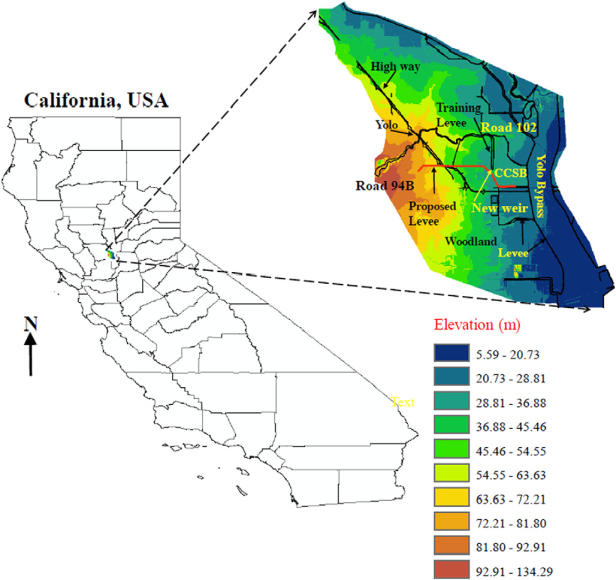
\includegraphics[width=0.8\textwidth]{location.png}
    \caption{Location of the study area in Northern California.}
    \label{fig:location}
\end{figure}

\section{Results and Key Findings}

\subsection{Flood Inundation Dynamics}
\hspace*{0.5cm}Under the current condition, the 10-year flood generated minimal overbank flow, with no water entering the CCSB. The 50-year flood caused limited inundation but did not activate the proposed inlet weir. In contrast, the 100- and 200-year floods produced significant overbank flow, submerging large portions of the CCSB and floodplain.

The alternative modification reduced flood risk south of the new levee, safeguarding urban and industrial zones. However, it increased water depths upstream: the 200-year flood elevated depths by 0.1–0.5 m in the CCSB and up to 2.5 m near the new levee. This trade-off underscores the challenge of protecting downstream areas while exacerbating upstream flooding.

\subsection{Sediment Transport and Trapping Efficiency}
\hspace*{0.5cm}Sediment trapping efficiency improved with flood magnitude under both scenarios. For the current condition, efficiency rose from 80\% (10-year flood) to 93\% (200-year flood) across the full domain, driven by sediment deposition in overbank areas. The CCSB alone trapped 31–66\% of sediment, with higher retention during larger floods due to increased coarse sediment (gravel, sand) delivery.

The alternative modification enhanced sediment retention in the northern CCSB by redistributing flow after levee removal. Trap efficiency for the CCSB increased by 10–15\% compared to the current condition, particularly for silt and clay. However, over 90\% of sediment exiting the system remained clay-sized, highlighting persistent risks of mercury transport to downstream ecosystems.

\subsection{Morphological Changes}
\hspace*{0.5cm}Under the current condition, sediment deposition concentrated in the southern CCSB, reducing channel conveyance and increasing flood hazards over time. The 200-year flood deposited up to 1.2 m of sediment in this region, exacerbating long-term vulnerability.

The alternative modification shifted deposition patterns: northern CCSB deposition increased by 0.5–1.0 m during extreme floods, while southern deposition decreased by 0.3–0.8 m. This redistribution preserved channel capacity in the south but required frequent dredging in the north. Bed slope adjustments further influenced flow velocities, altering sediment transport pathways.

\subsection{Management Implications}
\hspace*{0.5cm}The study reveals critical trade-offs between flood protection and environmental goals. The alternative modification effectively shields urban areas but intensifies upstream inundation, raising equity concerns for communities near the new levee. Enhanced sediment trapping in the CCSB benefits mercury mitigation but requires costly infrastructure investments and ongoing maintenance.

Environmental agencies prioritize sediment retention to limit mercury dispersion, while local communities emphasize flood risk reduction. Balancing these objectives demands adaptive management: optimizing levee heights, inlet weir operations, and dredging schedules could reconcile competing interests. Additionally, the findings challenge traditional assumptions of static river morphology in flood modeling, advocating for dynamic, sediment-inclusive hazard assessments.

\section{Conclusion}
\hspace*{0.5cm}This research demonstrates the value of integrated hydrodynamic-sediment modeling in evaluating multi-objective flood management strategies. By quantifying how extreme floods reshape hydrology and morphology, the study provides a framework for decision-makers to weigh flood protection against environmental health. The proposed modification offers partial solutions but underscores the need for compromise: no single strategy fully addresses all risks. Future work should explore hybrid approaches, such as phased levee construction coupled with wetland restoration, to enhance resilience. Ultimately, the study advocates for policies that harmonize engineering interventions with ecological preservation, ensuring sustainable management of flood-prone river systems.

\newpage
\begin{thebibliography}{99} 
\addcontentsline{toc}{section}{References}

\bibitem{Robertson2014} Robertson, A. N., Jonkman, J., and Musial, W. (2014). \textit{OC4-DeepCwind Semi-Submersible Baseline Control System Design}. National Renewable Energy Laboratory (NREL), Golden, CO.

\end{thebibliography}

\end{document}